\chapter{Security Risk Management}
\section{What is Risk Management?}
In brief, Risk Management is about identifying threats (or hazards) directed toward the business, then quantifying both the impact and likelihood of the threat occurring.

Safety risk management is well understood and practised particularly in more dangerous industries such as construction and mining. It also has government backing with Work and Safety legislation.

Shown in Figure \ref{fig:Risk}, ISO30001:2018 is a popular international standard for risk management. It defines the following risk management process:
\begin{figure}[h] \label{fig:Risk}
	\centering
	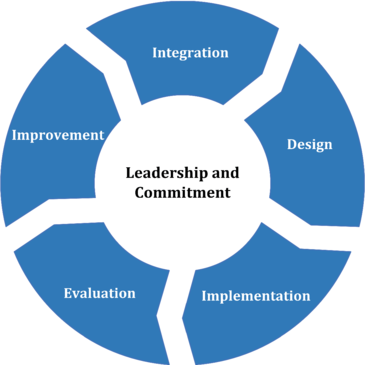
\includegraphics[width=0.45\textwidth]{./TeX_files/Framework1.png}	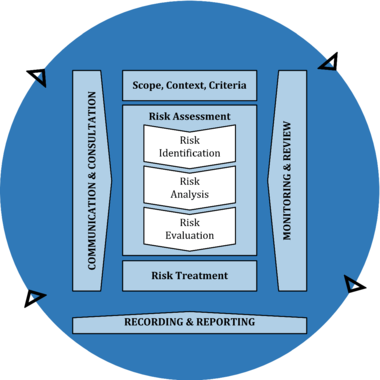
\includegraphics[width=0.45\textwidth]{./TeX_files/Process1.png}
	\caption{Risk Management Framework and Process}
\end{figure}

\begin{itemize}
	\item Communication;
	\item Defining Risk;
	\item Risk Assessment;
	\item Risk Treatment;
	\item Monitoring and Review;
	\item Recording and Reporting.
\end{itemize}
\section{Communication}
The objective of Communication is twofold. First it is an exchange of timely and accurate information with and between relevant internal and external stakeholders. Second it promotes an understanding of risk and how it is used as the basis for decision making prosecuting actions.
\section{Defining Risk}
The Risk Management program should define the organisational level applied to the risk management objectives e.g. Strategic, Program, Project, Operational.
Scope requires consideration of: a)Objectives and outcomes; b)Resources and responsibilities; c)Tools and techniques; d)Record keeping.

Furthermore, the program needs to define the method of risk evaluation. A simple example follows:
\begin{itemize}
	\item \textbf{Define Impact*}
	\subsubitem *Includes reputation damage resulting in financial loss
	\subitem Low=Financial loss less than 1 year earnings
	\subitem High=Financial loss more than 1 year earnings
	\item \textbf{Define Likelihood}
	\subitem Infrequent=Occurs less than once per year
	\subitem Often=Occurs more than once per year
\end{itemize}
\begin{table}[h]
	\centering
	\begin{tabular}{c|c|c}
	\textit{Risk Table} &\textbf{Low Impact} &\textbf{High Impact} \\
	\hline
	\textbf{Occurs Infrequently} &Low Risk &Medium Risk \\
	\textbf{Occurs Often} &Medium Risk &High Risk \\
	\end{tabular}
\end{table}
The example above defines consequences (Financial and reputational loss) and a quantifiable risk level (annual earnings). A larger risk definition will consider the organisations context - that is the wider external and internal factors within the operating environment. This is sometimes referred to as "Threat Surface". 
Finally, a risk management program needs to define the appetite for risk. How much risk is acceptable before the manage should pass the decision to act (or not act) to a higher authority.
\section{Risk Assessment}
Assessing risk encompasses the three processes of:
\begin{itemize}
	\item Identifying the risk source: Where does it come from? Where are we vulnerable? What is the threat environment?
	\begin{table}[h]
		\centering
		\begin{tabular}{c|c}
		\textbf{Tangible Risk Source} &\textbf{Intangible Risk Source} \\
		\hline
		\begin{minipage}{7cm}\subitem(Loss of) physical assets, including data or information asset stored computer disks.
		\subitem Also, negligent damage to third party assets including environment, property and people.
		\subitem Capability gaps.
		\subitem Change in operating environment and/or external events.
		\end{minipage} &\begin{minipage}{6cm}\subitem Usually socio-economic or legal risk which may impede achieving the objective. E.g. Public opposition could lower reputation and result in boycot, or legal actions.
		\subitem Knowledge gaps.
		\subitem Change in operating context.
		\end{minipage} \\
		\hline
		\end{tabular}
	\end{table}
	\item Determine the consequences if risk materialises: What will happen? How bad will it be? Can our objectives still be achieved? How likely is it? Are there any mitigating factors (controls)?
	\item Evaluation: Compare the assessed level of risk against the organisations risk thresholds to inform the decision to act (or not) and the amount of effort or resource put to mitigating the risk.
	A decision to act (or not) will result in developing a risk treatment plan.
\end{itemize}
\section{Risk Treatment}
\section{Monitoring and Review}
\section{Recording and Reporting}
